 \documentclass[%
 aps,
 prl,%
 amsmath,amssymb,
%preprint,%
 reprint,%
%author-year,%
%author-numerical,%
]{revtex4-1}

\usepackage{graphicx}% Include figure files
\usepackage{dcolumn}% Align table columns on decimal point
\usepackage{bm}% bold math
%My packages start
%\usepackage{subfig}
\usepackage{multirow}					
\usepackage{array}
%\usepackage{booktabs}
\usepackage{footnote} 
\newcommand{\angstrom}{\text{\normalfont\AA}}
\usepackage{booktabs}
\usepackage{float}
\usepackage{mathtools}
\usepackage{color}
\newcommand{\comment}[1]{\noindent \textcolor{blue}{#1}}
%My packages end
%\usepackage[mathlines]{lineno}% Enable numbering of text and display math
%\linenumbers\relax % Commence numbering lines

\begin{document}

\title[]{Accelerating atomic structure search with cluster regularization}% Force line breaks with \\

\author{K.\ H.\ S{\o}rensen}
\author{M.\ S.\ J{\o}rgensen}
\author{A.\ Bruix}
\author{B.\ Hammer}
\email{hammer@phys.au.dk}
\affiliation{ 
Department of Physics and Astronomy, and Interdisciplinary Nanoscience Center (iNANO), Aarhus University, DK-8000 Aarhus C, Denmark.
}
% \homepage{phys.au.dk}
 
\date{\today}% It is always \today, today,
             %  but any date may be explicitly specified

\begin{abstract}
We present a method for accelerating the global structure optimization
of atomic compounds. The method is demonstrated to speed up the
finding of the anatase TiO$_2$(001)-(1$\times$4) surface
reconstruction within a density functional tight-binding theory
framework using an evolutionary algorithm (EA). As a key element of the
method, we use unsupervised machine learning techniques to categorize
atoms present in a diverse set of partially disordered surface structures
into clusters of atoms having similar local atomic
environments. Analysis of more than 1000 different structures shows
that the total energy of the structures correlate with the summed
distances of the atomic environments to their
respective cluster centers in feature space, where the sum runs over all atoms in each
structure. Our method is formulated as a gradient based minimization
of this summed cluster distance for a given structure and alternates
with a standard gradient based energy minimization. While the latter
minimization ensures local relaxation within a given energy basin,
the former enables escapes from meta-stable basins and hence increases
the overall performance of the global optimization.
\end{abstract}

\pacs{Valid PACS appear here}% PACS, the Physics and Astronomy
                             % Classification Scheme.
\keywords{}%Use showkeys class option if keyword
                              %display desired
\maketitle

\section{\label{sec:introduction}Introduction}
In computational materials science, knowing the atomic structure of a
given molecule, atomic cluster or solid compound is a prerequisite for
further prediction of electronic and thermodynamic properties of such
a substance.\cite{} In the emerging fields of combinatorial chemistry and
high-throughput computational screening of materials,\cite{} the use of local
relaxation of probed structures is often sufficient since libraries of
molecular building blocks and crystal structures can be used to direct
the starting points for the searches.\cite{} However, many problems exist for
which the structural motifs in the sought-after structures have no
analogues in known structures, and where global optimization must be
employed. A prominent example of this is that of surface relaxations,
which often exhibit structural motifs that are unique to a chemical
composition, crystaline polymorph, and surface orientation. Monomeric
Si adatoms and restatoms and zig-zagging Si-dimers do for example evolve at the
Si(111)-(7$\times$7) and Si(001)-c(4$\times$2) surfaces,\cite{} respectively, but
are otherwise not present in bulk Si or bulk-truncated Si surfaces. Likewise,
rutile and anatase TiO$_2$ single-crystal surfaces are known to exhibit
reconstructions and ad-structures,\cite{} that have no equivalent in any TiO$_2$ bulk or surface systems.

Many strategies exist for performing global optimization in
conjunction with model potentials or first-principles total energy
frameworks. Among these, stoichastic methods such as random search\cite{} and
basin hopping (BH)\cite{} are widely used and more advanced methods based on
evolutionary algorithms (EA) are becoming increasingly popular.\cite{} Common
to these methods is the need for the perturbative update steps
followed by local relaxation and evaluation of whether or not to
retain the new structure. The nature of the perturbation steps ranges
from a mere rattling of the atomic positions to highly advanced
cross-over operations in which the atomic structures of several known
systems are combined.\cite{} The exploration of configuration space is
ensured by the very stochastic nature of these updates, yet updates
that are too random will lead to rejection of the locally
relaxed structure too often and hence cause slow convergence. The atomic
displacement amplitude in a rattling update is a good example of
this. The amplitude must be kept small and sometimes only apply to a
subset of the atoms, as the new structural candidate otherwise become
too unstable.

The present work aims at formulating a means of performing a random
update in a way that optimizes the chances of finding more stable
structural candidates in subsequent local relaxation steps. The method
proposed starts from assigning every atom in a given structure to a
cluster of similar atoms present in a reference set of structures.
The similarity is measured as the distance in a feature space, chosen in this work
sufficiently simple that it can be illustrated. With every atom
assigned to a cluster, we evaluate for a given structure the sum of
the distances space of the atoms from their respective
cluster centers in feature. This structure specific scalar measure of distance to
cluster centers is demonstrated to correlate with the structure
stability -- the lower the distance measure, the more likely that the
structure is more stable. As a consequence, minimizing the cluster distance measure
contains an element of bringing a structure into a region of
configuration space that is expectedly more stable. The minimization
can be done by moving opposite to an analytic gradient and has
potential to take a structure out of local energy minima, since the
cluster distances are measured in a space that is complementary to that of the
energy landscape. We refer to our method as the
\textit{cluster regularization method} as it penalizes large
distances of cluster members to their cluster centers.

The paper is outlined as follows: In the Methods section we present
the computational setup, outline the reference method used, and
describe the required machine learning components of our method,
including the choice of feature vector and the clustering technique.
In the New Method section we analyse some data and formulate the cluster
regularization method. In the Results and Discussion
section, the method is used in full scale global optimization in
search for the anatase TiO$_2$(001)-(1$\times$4) surface
reconstruction. This section demonstrates the usefulness of the method
and further investigates its efficacy as the number of unknown atomic
position is increased in the global optimization.

\section{Method}

\subsection{density functional tight-binding theory}
Density functional tight-binding (DFTB) theory calculations were
performed for TiO$_2$ structures using parameters from ref \cite{}.
With this description, bulk anatase TiO$_2$ has lattice parameters of
XX and XX {\AA} that compare well with the experimental values of XX
and XX {\AA}. DFTB calculations have previously been conducted
successfully for the study of XX and XX.  In the present work, we
employ 2D periodic super cells accomodating the anatase TiO$_2$(001)
surface with (4$\times$1) periodicity. Slabs of three different
thicknesses were considered, containing two, three, or four layers of
atoms. The three-layer system is illustrated in Figure \ref{figintro},
showing the template of four static TiO$_2$ units, two examples of
disordered structures with nine extra TiO$_2$ units added, and the
global minimum energy structure with three well ordered atomic layers
and one extra row of TiO$_2$ protruding out of the surface.
\begin{figure}[tb]
    \centering
    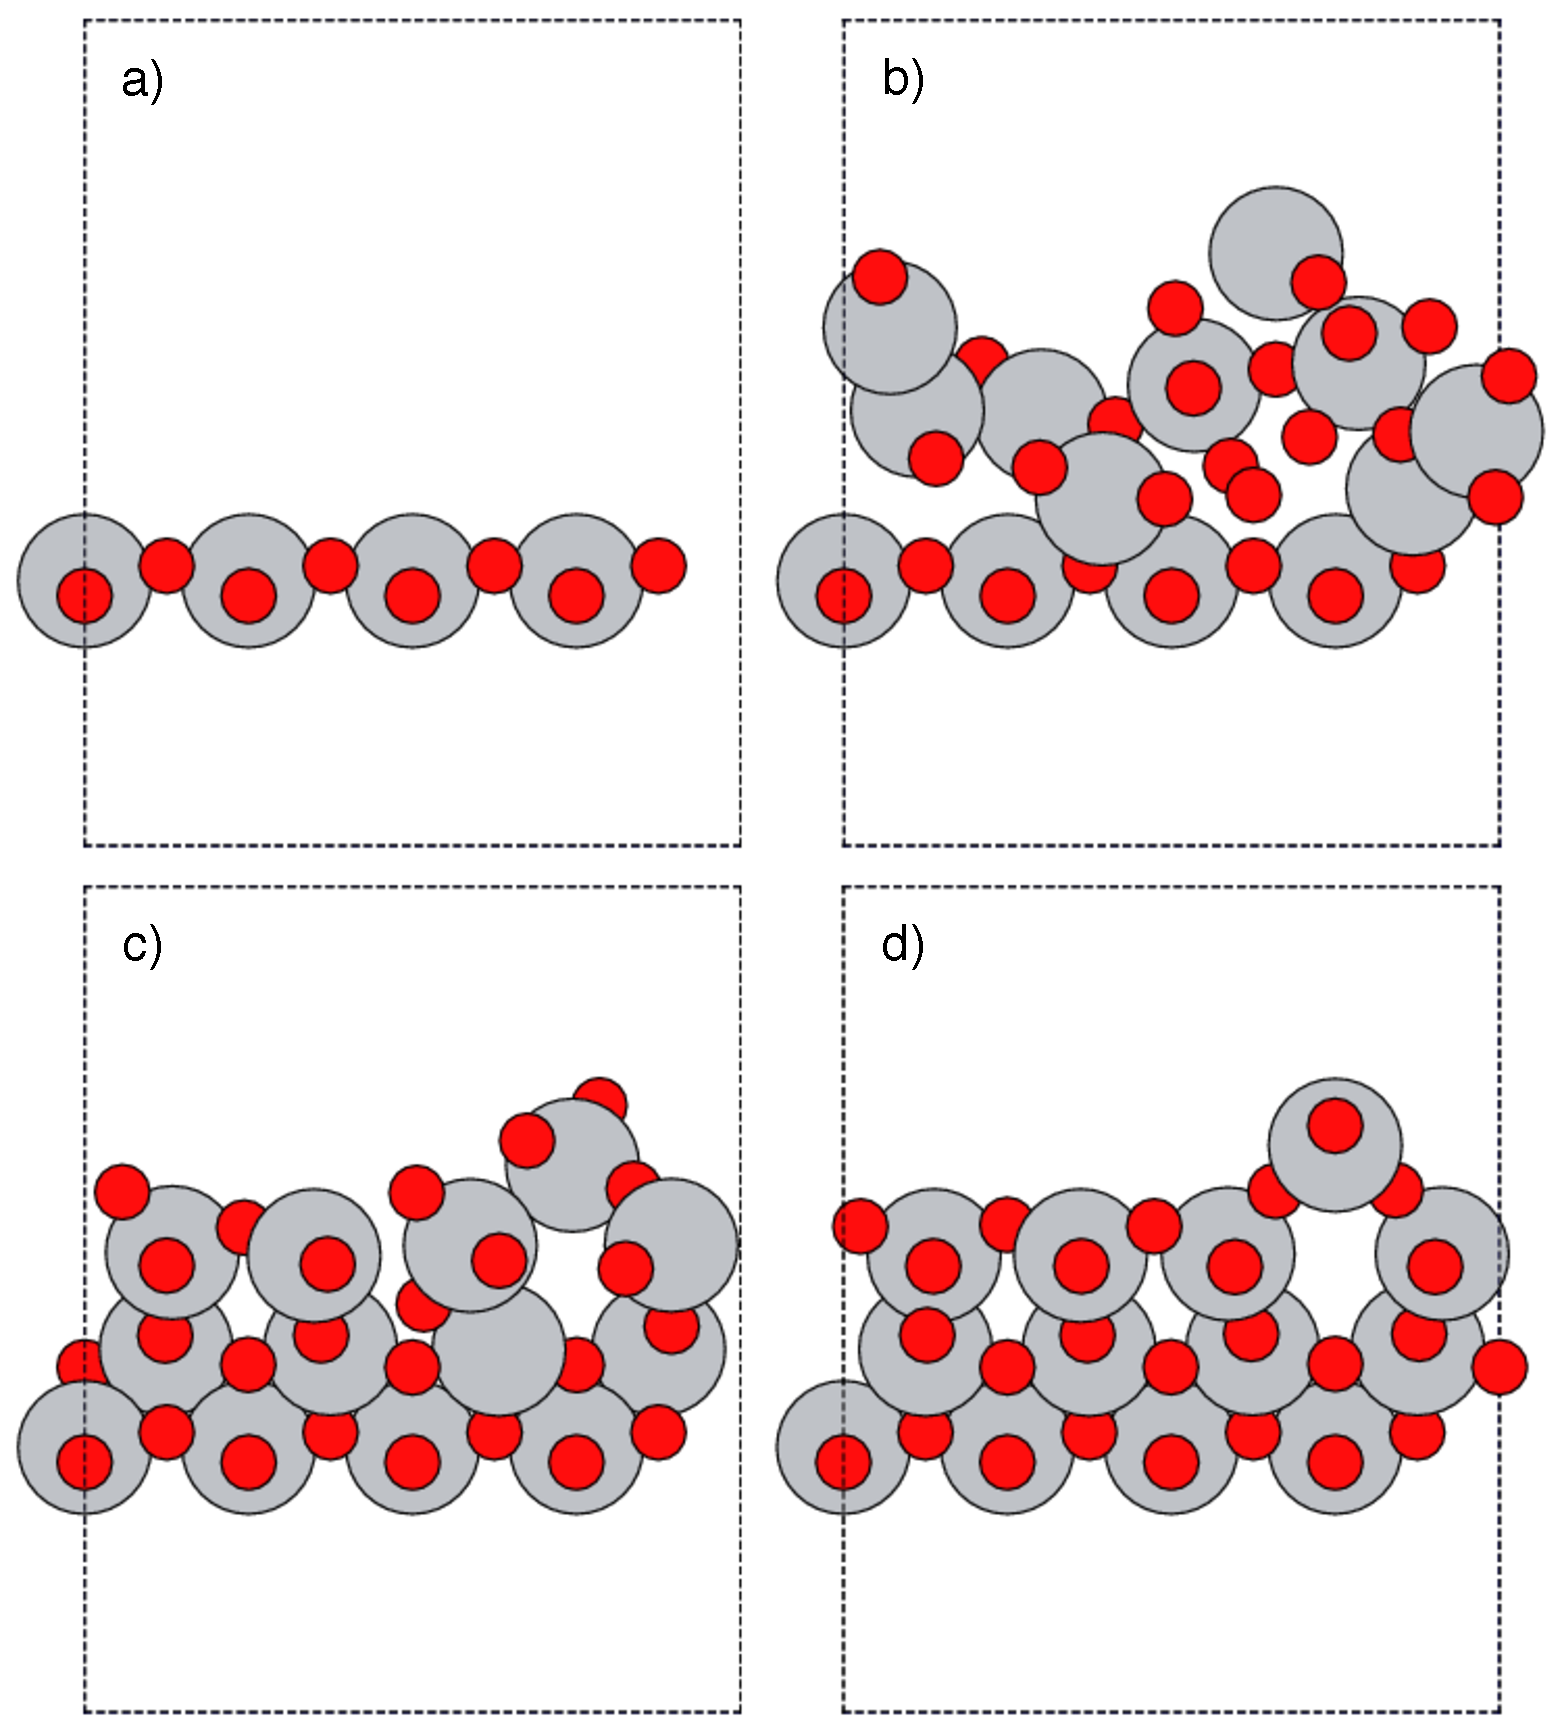
\includegraphics[width=1.0\columnwidth]{fig1-intro.pdf}
    \caption{Side views of computational cells with Ti$_{n}$O$_{2n}$ structures.
      Small red spheres: Oxygen, large grey spheres: Ti.
      a) The template of four TiO$_2$ units.
      b-c) Two examples of intermediate structures from an evolutionary search. Nine TiO$_2$ units
      have been placed on the template.
      d) The sought-after global minimum structure for the anatase TiO$_2$(001)-(1$\times$4) surface.
    }
    \label{figintro}
\end{figure}

\subsection{Evolutionary algorithm}
The disordered structures in Figure \ref{figintro} are snapshots from
search runs performed with the evolutionary algorithm (EA) available
in the Atomic Simulation Environment (ASE)\cite{ase2}.  The EA
iteratively improves the positions of the atoms atop the template
structure (Figure \ref{figintro}a) using cross-over operations
combining two parent structures or mutation operations applied to
single parent structures. The resulting offspring structures undergo
local relaxation within DFTB following the atomic forces (i.e.,\ the negative of
the energy gradient). A population of $N_\mathrm{pop}=20$ parent structures
is maintained, and new candidates are tested one at a time.
The relaxed offspring structures are included in the population
according to their fitness evaluated as the negative of the DFTB energy.
More details on the EA are given in refs \cite{Vilhelmsen2012} and \cite{Vilhelmsen2014}.

The cluster regularization method proposed in this work is implemented
as a mutation operation and its usefulness is gauged by comparing an
EA search where this mutation is used either exclusively or
occasionally to a benchmark EA search, where it is not used at all. We
also test the method in a basin hopping (BH) framework,\cite{} in which some
perturbing update step alternates with a local energy relaxation step.

\subsection{Machine learning techniques}
Our method uses two components of general machine learning techniques:
the representation of the data with a feature vector, and the
classification of the data utilizing clustering methods.

\subsubsection{Feature vector}
Feature vector representations of the atomic structure of molecules,
clusters, and solids serve the general purpose of introducing
invariance with respect to symmetries obeyed by the total energy
operator, i.e.\ the Hamiltonian. The symmetries are those of translation
or rotation of the entire system or the permutation of the order of
atoms with the same chemical identity. Without a symmetry invariant
representation, e.g.\ using cartesian coordinates, a certain structure
will have a finite distance to for instance a translated copy of
itself, even though the two systems will have identical physical
properties. However, when measured in a proper feature space, two such
structures may have a zero distance.

A large and increasing number of feature vector formulations appear in
the chemical physics literature. Global feature vectors of entire
systems include the bag-of-bonds\cite{} and fingerprint\cite{} feature
vectors, that are composed of either a sorted list or a histogram of
all interatomic distances in the compounds, but also more
sophisticated methods such as the Coulomb matrix\cite{} have been
proposed.

Atom-specific feature vectors representing the local
chemical environments of the atoms in a compound structure are
particularly abundant in the literature. Such feature vectors are usually
formulated in internal coordinates and therefore have the translational
and rotational invariance conveniently build in by construction. The Behler-Parrinello (BP)
symmetry function formulation\cite{} stand out as a seminal
contribution, yet one with rather many parameters to be chosen by the
user. With BP symmetry functions, each atom is represented by a selection
of 2-body distance terms and 3-body angular terms. All terms are
attenuated with a cutoff function that ensures a smooth decay to
zero at a set cutoff distance.  Recently, more advanced atom-specific feature vectors
have been developed for which higher-order interactions (e.g.\ 4-atom torsion angles) are included.
Such feature vectors have proven superior in reproducing energies,
HOMO-LUMO gaps, polarizations, and a number of other properties for a
diverse set of molecules.\cite{}

In the present work we adopt an exceedingly simple atom-specific
feature vector with only three components:
\begin{equation}
\mathbf{f}_i=\left[Z_i,\rho_i^{Z^\mathrm{O}},\rho_i^{Z^\mathrm{Ti}}\right]\label{eq_feature}
\end{equation}
where $Z_i$ is the atomic number of atom $i$, while
$\rho_i^{Z^\mathrm{O}}$ and $\rho_i^{Z^\mathrm{Ti}}$ are measures for
atom $i$ of the density of neighboring oxygen and titanium atoms,
respectively. These densities are inspired by the radial symmetry
functions of Behler \textit{et al.}\cite{}. For a discussion on this see the work of Botu
and Ramprasad \cite{Botu2015}. In our work we use:
\begin{equation}
\rho_i^Z = \sum_{j\ne i,Z_j=Z} e^{-r_{ij}/\lambda}g_c(r_{ij})  \label{eq1}
\end{equation}
where $Z$ is either $Z^\mathrm{O}$ or $Z^\mathrm{Ti}$, $j$ runs over
all atomic indices, $Z_j$ is the atomic number of the $j$'th atom, $r_{ij}$ is the distance $|\mathbf r_{ij}|=|\mathbf r_j-
\mathbf r_i|$ from the $i$'th to the $j$'th atom, and
$\lambda=1$ {\AA} is a chosen length scale. $g_c$ is a cut-off
function given by:
\begin{equation}
g_c(r)=
\left\{\begin{array}{ll}
\frac{1}{2}{\cos(\pi \frac{r}{r_c})+\frac{1}{2}},&r<r_c\\
\\
0,&r\ge r_c
\end{array}
\right.
\end{equation}
which ensures that the densities vanish algebraically at the cut-off
radius, $r_c$. For $r_c$ we use 11.9 {\AA} which was determined in a parameter search detailed below.
Owing to the presence of $g_c$, the sum in Eq.\ (\ref{eq1}) needs
in practice only to run over nearest neighbors to atom $i$.

\subsubsection{Clustering}
Molecular and chemical physicists are often faced with vast configuration spaces when studying the structures of chemical compounds. Clustering techniques have proven valuable tools when trying to find reoccurring structural moieties \cite{Gilbert2006}, especially in combination with molecular dynamics where thousands of structure trajectories are generated \cite{Duan2010,Chema2002}. Clustering has also previously been used to aid global structure optimization \cite{Jorgensen2017}.

The clustering method used is this study is k-means with two
modifications. The first is a modification to avoid generating empty
clusters \cite{Malay2009} and the second modification is the use of
k-means++ cluster initialization. Unless otherwise stated, we use a fixed number
of cluster centers, $N_c=5$.

Whenever clustering of atom-specific feature vectors has been
performed, a set of resulting cluster centers,
$\left\{\mathbf{c}_k\right\}$, will be known. Representing by $k(i)$ the
index of the cluster center that a given atom $i$ belongs to, we can
now evaluate the sum of all cluster distances for a given structure accoring to:
\begin{equation}
D_S = \sum_{i \in S} \left|\mathbf f_i- \mathbf c_{k(i)}\right| \label{eq4}
\end{equation}
where $S$ is the structure (a list of atoms). Note that $D_S$ is a
scalar number, which in principle exists for any conceivable set of
$N$ atomic positions. As such, a continuous
"cluster-distance"-landscape exists in $\mathbb{R}^{3N}$, and the
atomic positions may be changed towards an overall smaller cluster
distance by following the negative of the gradient of the cluster distance with
respect to the atomic positions, $\mathbf{R}$:
\begin{equation}
-\nabla_\mathbf{R} D_S = -\sum_{Z \in \{Z^O,Z^{Ti}\}}\sum_{i \in S} \left(\nabla_\mathbf{R}\rho_i^Z\right)
\frac{\partial}{\partial\rho_i^Z}\left|\mathbf f_i- \mathbf c_{k(i)}\right|,
\end{equation}
$$
XXXXX a missing factor?
$$
where the cluster centers are kept fixed.  This is analogous to the
atomic forces directing the minimization of the energy in the energy
landscape.

\section{Feature space analysis}

Owing to its low dimensionality, the atom-specific feature vector can
be illustrated in two-dimensional scatter plots. This is done in
Figures \ref{fig_global} and \ref{fig_feature} where features
pertaining to oxygen and titanium atoms are shown in red and grey
color, respectively.  The two axes in the plots are the
$\rho^{Z^\mathrm{O}}$ and $\rho^{Z^\mathrm{Ti}}$ densities.  In
Figure \ref{fig_global}, the atomic structure considered is that of the
three-layer global minimum energy structure introduced in
Figure \ref{figintro}d. The figure shows that strong correlations exist
for the features. Features for oxygen atoms lie on one line, while
features for titanium atoms lie on another. Within each line the 26
data points for oxygen atoms and 13 data points for titanium atoms
further appear in a number of clusters. The lines reflect that in this
global minimum energy structure the atoms have a nearly constant
ratio of neighboring atoms of the two possible types.

\begin{figure}[tb]
    \centering
    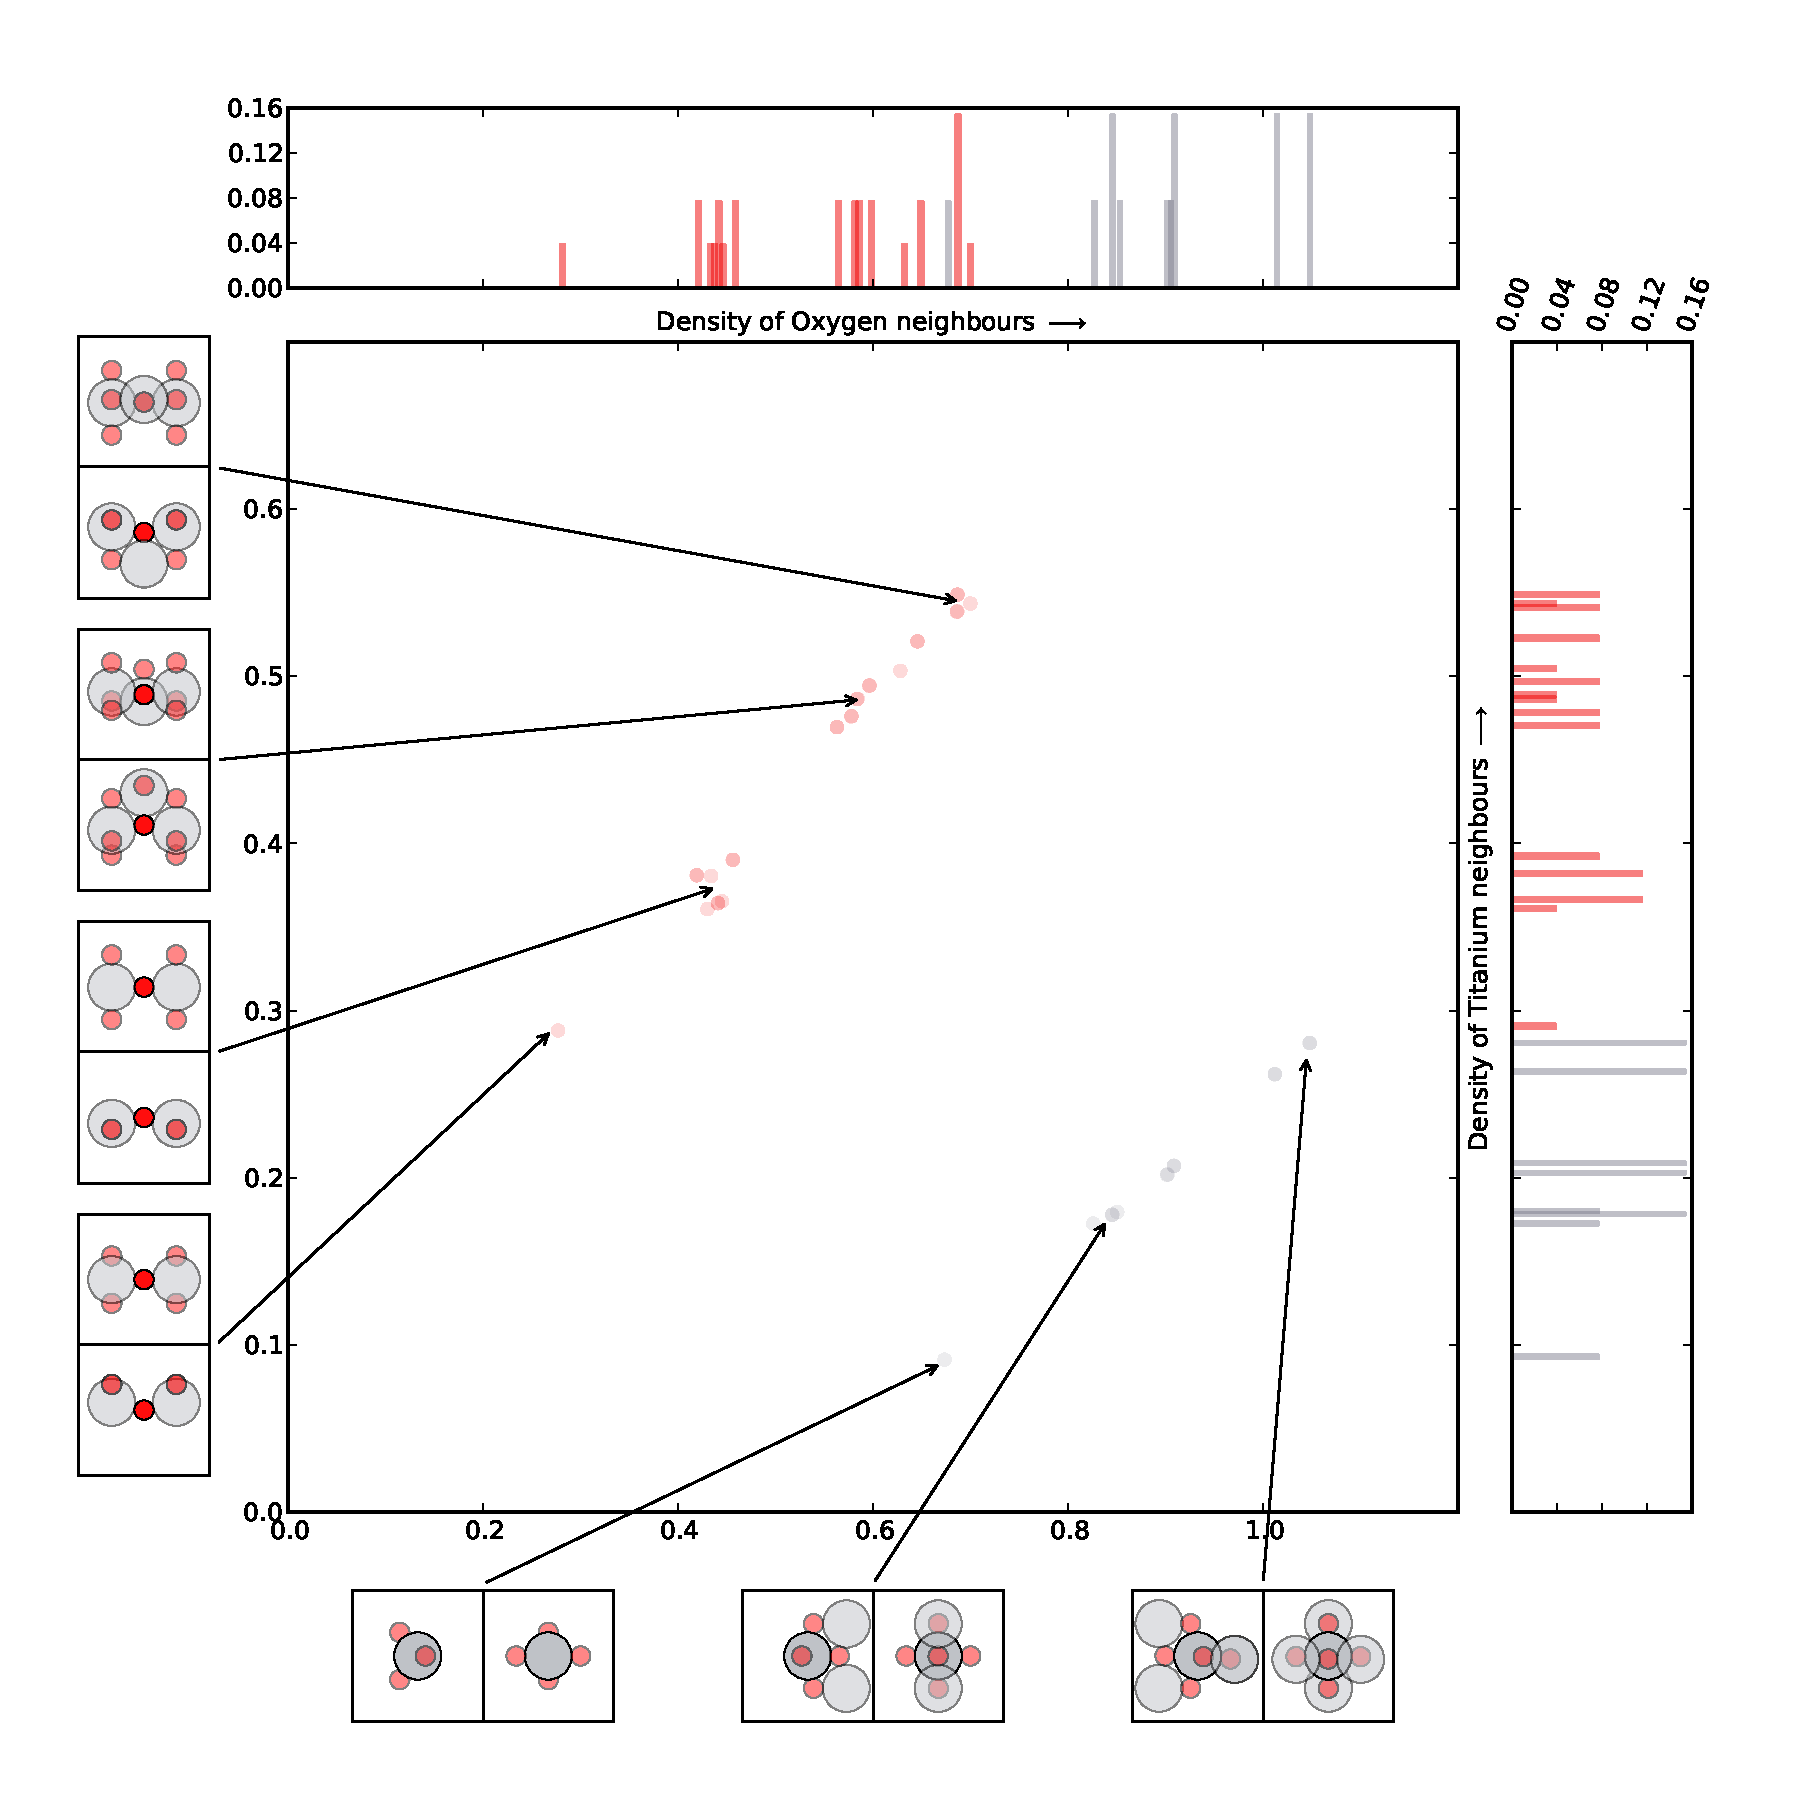
\includegraphics[width=1.0\columnwidth]{fig2-gm_scatterplot.pdf}
    \caption{Visualization of global minimum for Ti$_{13}$O$_{26}$ structures in feature space}   
    \label{fig_global}
\end{figure}



\begin{figure}[tb]
    \centering
    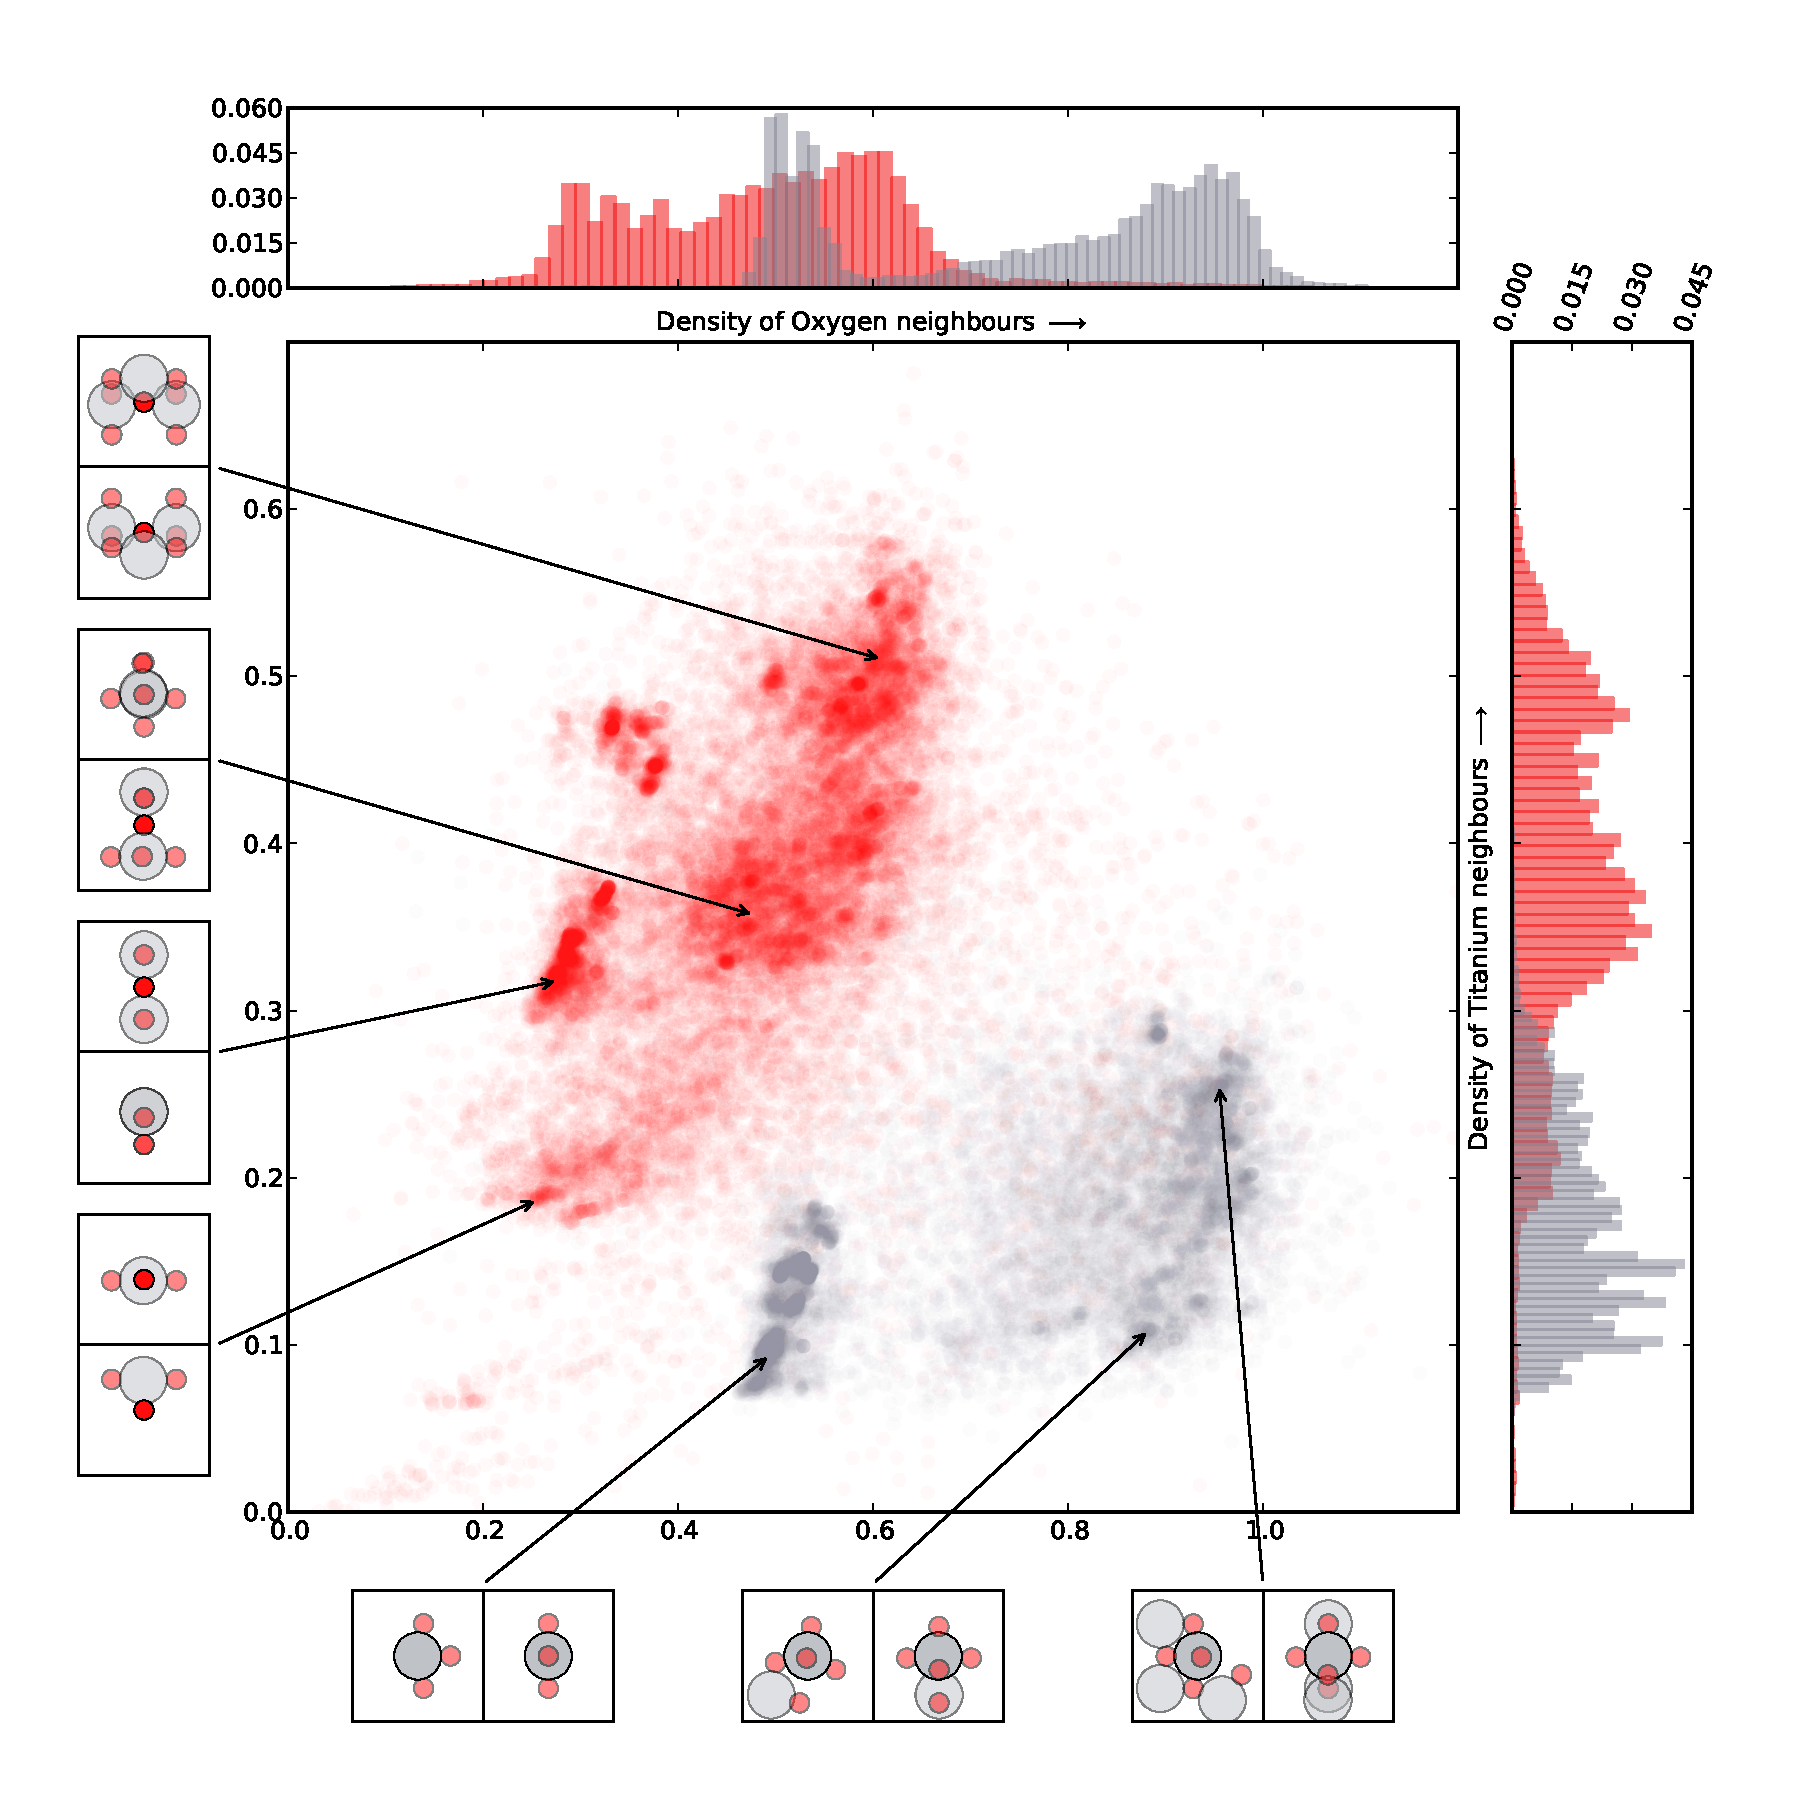
\includegraphics[width=1.0\columnwidth]{fig3-scatterplot.pdf}
    \caption{Visualization of atoms from 1019 Ti$_{13}$O$_{26}$ structures in feature space}   
    \label{fig_feature}
\end{figure}

Figure \ref{fig_feature} presents the distribution of atomic features
for the 26+13 atoms in about 1000 different structures of the
three-layer system. The structures are taken from several EA searches
and have been filtered so that they can be considered distinct
structures. The wide distribution of the feature vectors for general
structures as opposed to the highly ordered features for the global
minimum energy structure indicate that despite its simplicity the
feature vector holds great potential to capture variations in local
structure present in the disordered structures. The feature vector is
clearly not unique as for example an atom with a single close neighbor may have the
same feature vector as an atom with two more distant neighbors. However, in the
current context, this is not of importance, since the rich variety in feature
vectors over a real data set as seen in Figure \ref{fig_feature} is the
desired property.

\begin{figure}[tb]
    \centering
    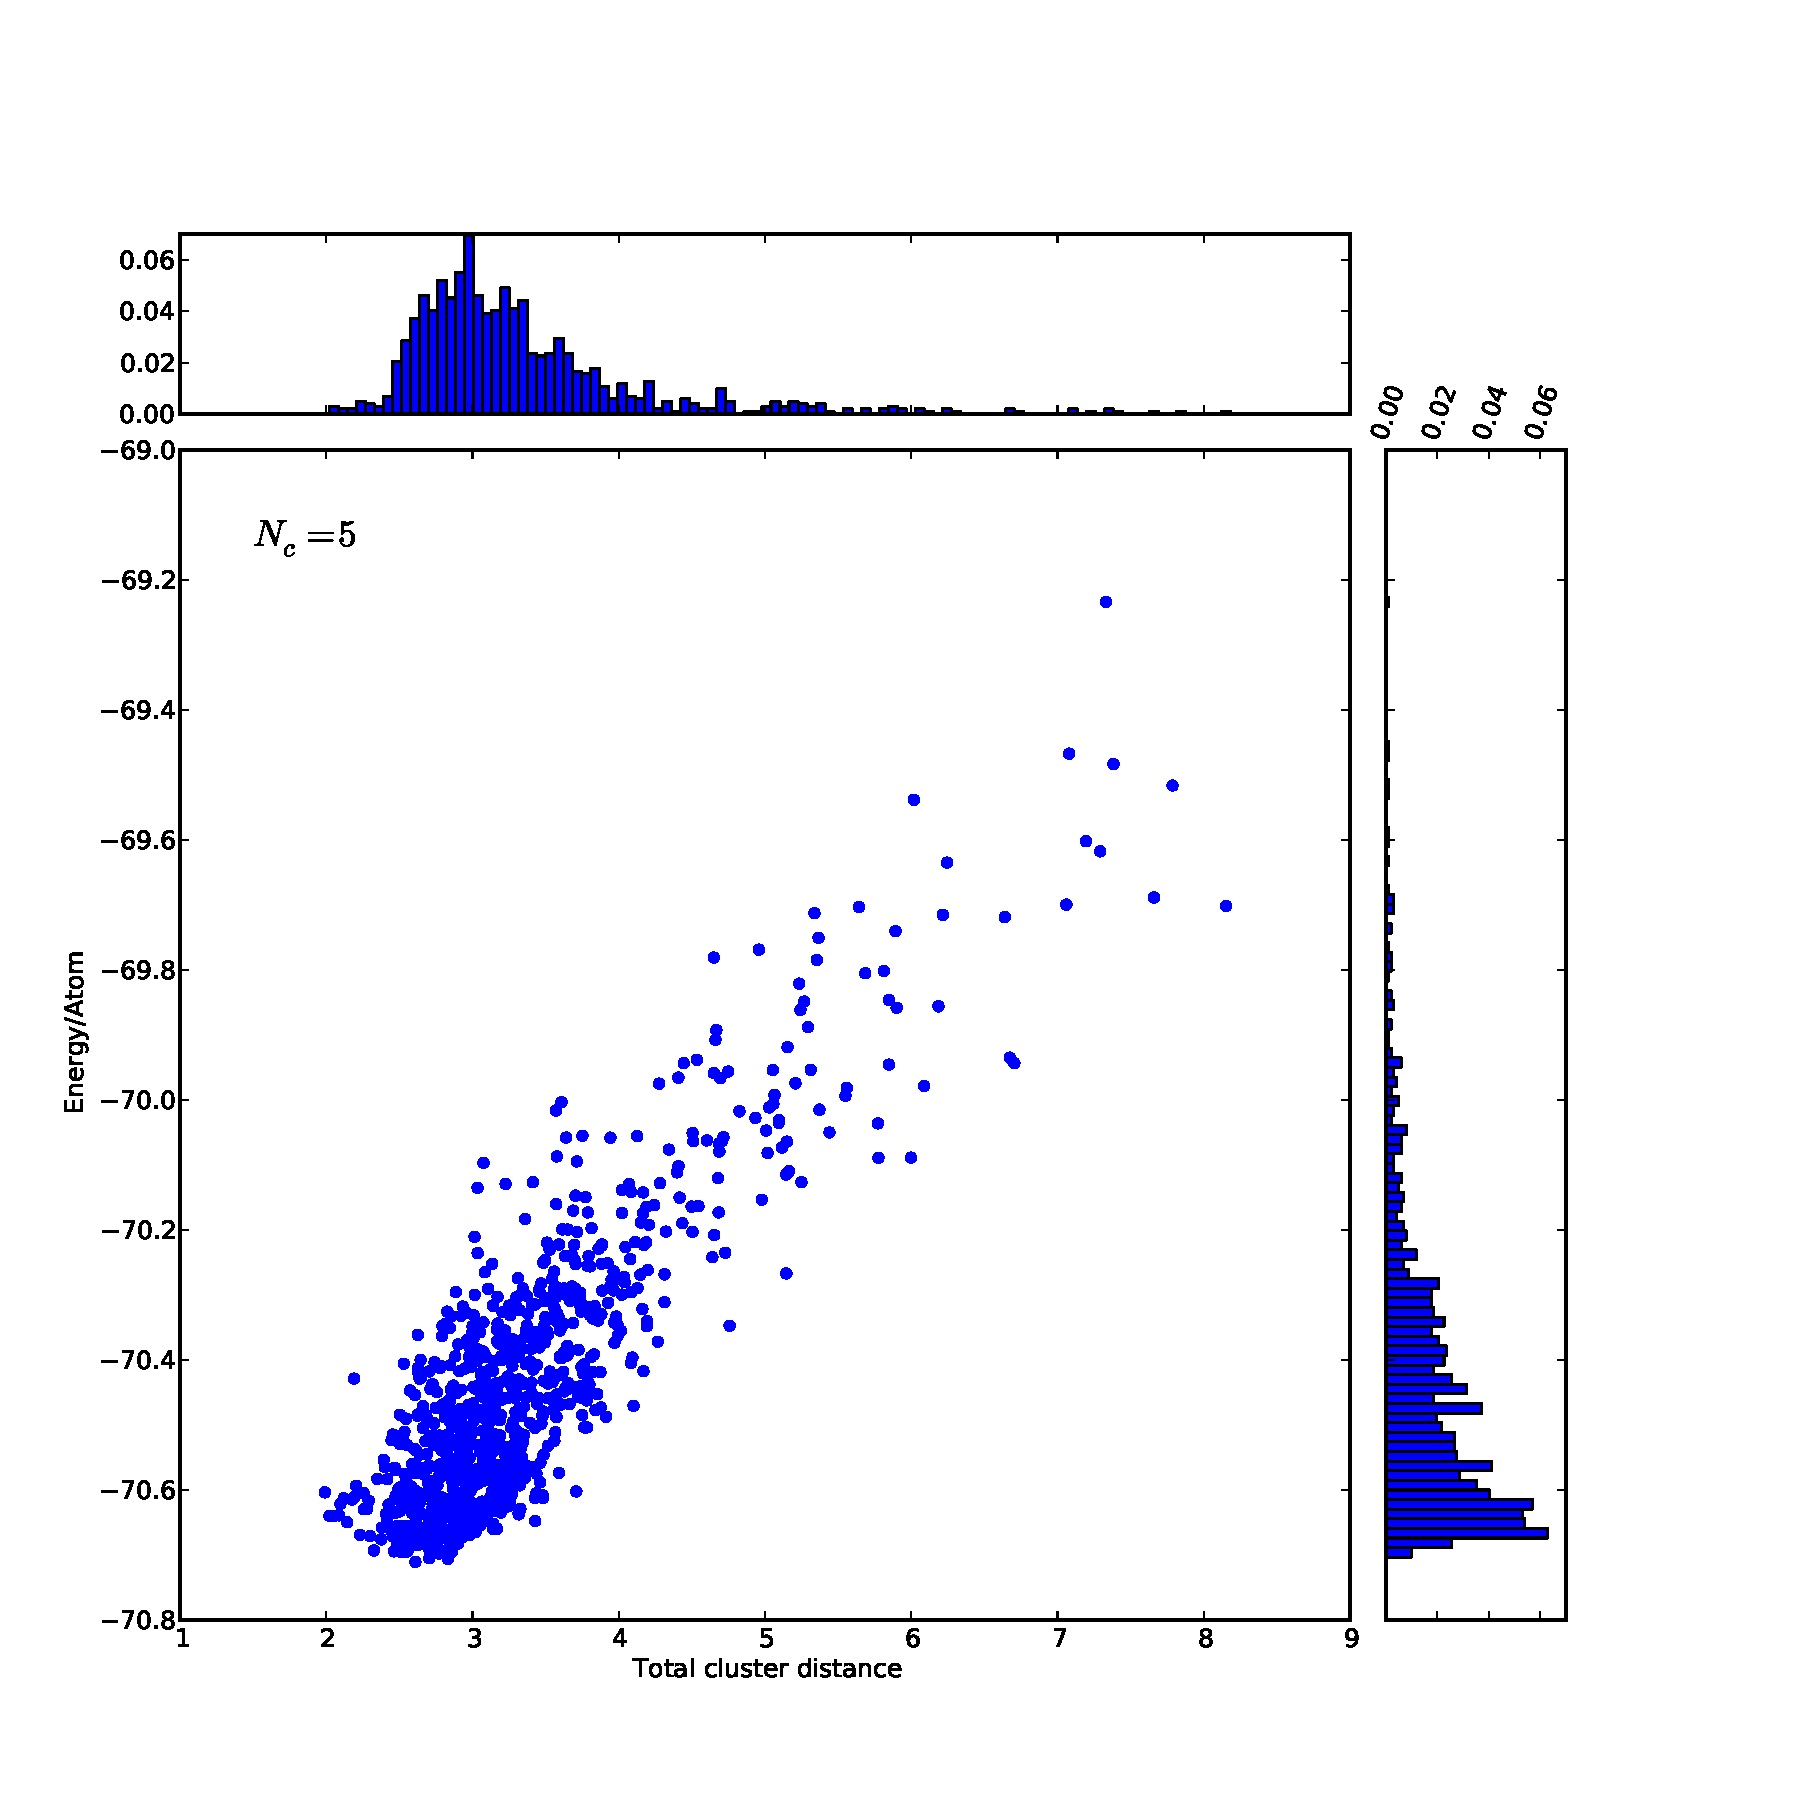
\includegraphics[width=1.0\columnwidth]{fig4-correlation.pdf}
    \caption{Cluster distance vs. energy correlation}
    \label{fig_corr}
\end{figure}

A strong correlation between the total
cluster distance, $D_S$, and the total DFTB energy,
$E_S^\mathrm{DFTB}$, is revealed when
clustering of the atomic feature vectors presented in
Figure \ref{fig_feature} is performed. The correlation illustrated in
Figure \ref{fig_corr} may in part be explained by the
general observation that nature often favors high
symmetry\cite{Pikard2011}, i.e.\ structures with low energy often have
recurring atomic motifs. A single crystal is an obvious example of
this, since all the atoms assume the same local
environments. In fact, for bulk anatase TiO$_2$, the scatter plot similar to
Figures \ref{fig_global} and \ref{fig_feature} only contains just one point
for each of the two chemical elements, oxygen and titanium. Hence, with
two cluster centers, the total cluster distance for bulk anatase TiO$_2$ would be zero. In our
case, the slab geometry used is causing the presence of two surfaces
that act to give several possible motifs, as evidenced for the global
minimum energy structure by Figure \ref{fig_global}, where now the total cluster
distance becomes finite, reflecting the surface energy cost. For any
disordered slab structure, the feature vectors scatter even more and the cluster distance increases
further at the same time as the total energy of the structure
raises above that of the global minimum energy structure (Figure \ref{fig_corr}).

\section{Cluster regularization method}

\begin{figure}[tb]
    \centering
    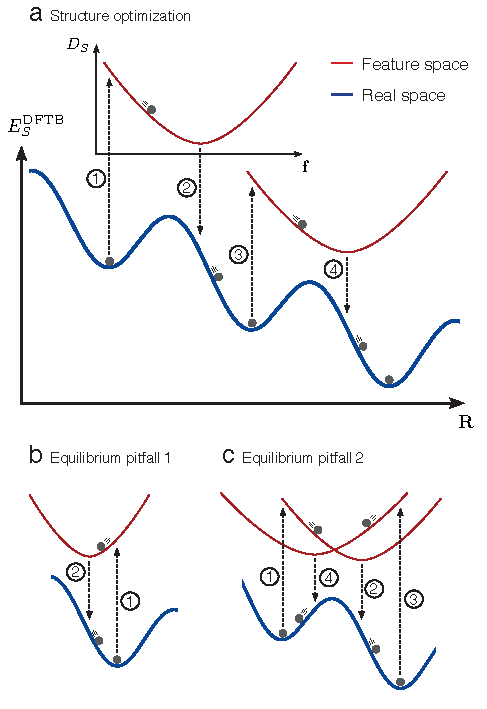
\includegraphics[width=1.0\columnwidth]{schematic.pdf}
    \caption{a) Structure optimization via alternation between minimization in real space and feature space. b+c) Situations where the structure is stuck in one or more real space local minima due to an equilibrium between minima in real space and feature space.}
    \label{fig_schem}
\end{figure}

The observed correlation between energy and cluster distance forms the
basis for our new method for perturbing an atomic structure in the
search for the global minimum energy structure. The method simply
performs a local minimization of the cluster distance for fixed
cluster centers. I.e.\ structures subjected to the method undergo
regularization with respect to their cluster distance measure. The
regularization takes place as a gradient based optimization using
standard techniques. There is no guarantee or even expectation that the
cluster regularization will directly perturb a given structure towards
a lower energy structure, but the cluster distance-energy correlation
in Figure\ \ref{fig_corr} is suggestive that when moved according to (minus) the cluster distance gradient, a given structure may leave a meta-stable basin
region of the energy landscape and move into a more favorable
basin in the energy landscape. The principle of the method is illustrated
schematically in Figure \ref{fig_schem}a, where transformations between real space and feature space enables the structure to escape local minima. Note that a local minimum in real space is only escaped if the local minimum in feature space takes the structure to another energy basin in real space. If this is not the case, the optimization will enter an equilibrium state between real space and feature space, and thus the structure will become trapped in one or more energy basins (Figures \ref{fig_schem}b and c). In the following, we demonstrate the usefulness of
the method in two different setups,
either as the perturbation step in a basin hopping (BH) framework or as a
possible perturbation step in an evolutionary search.

\begin{figure*}[tb]
    \centering
    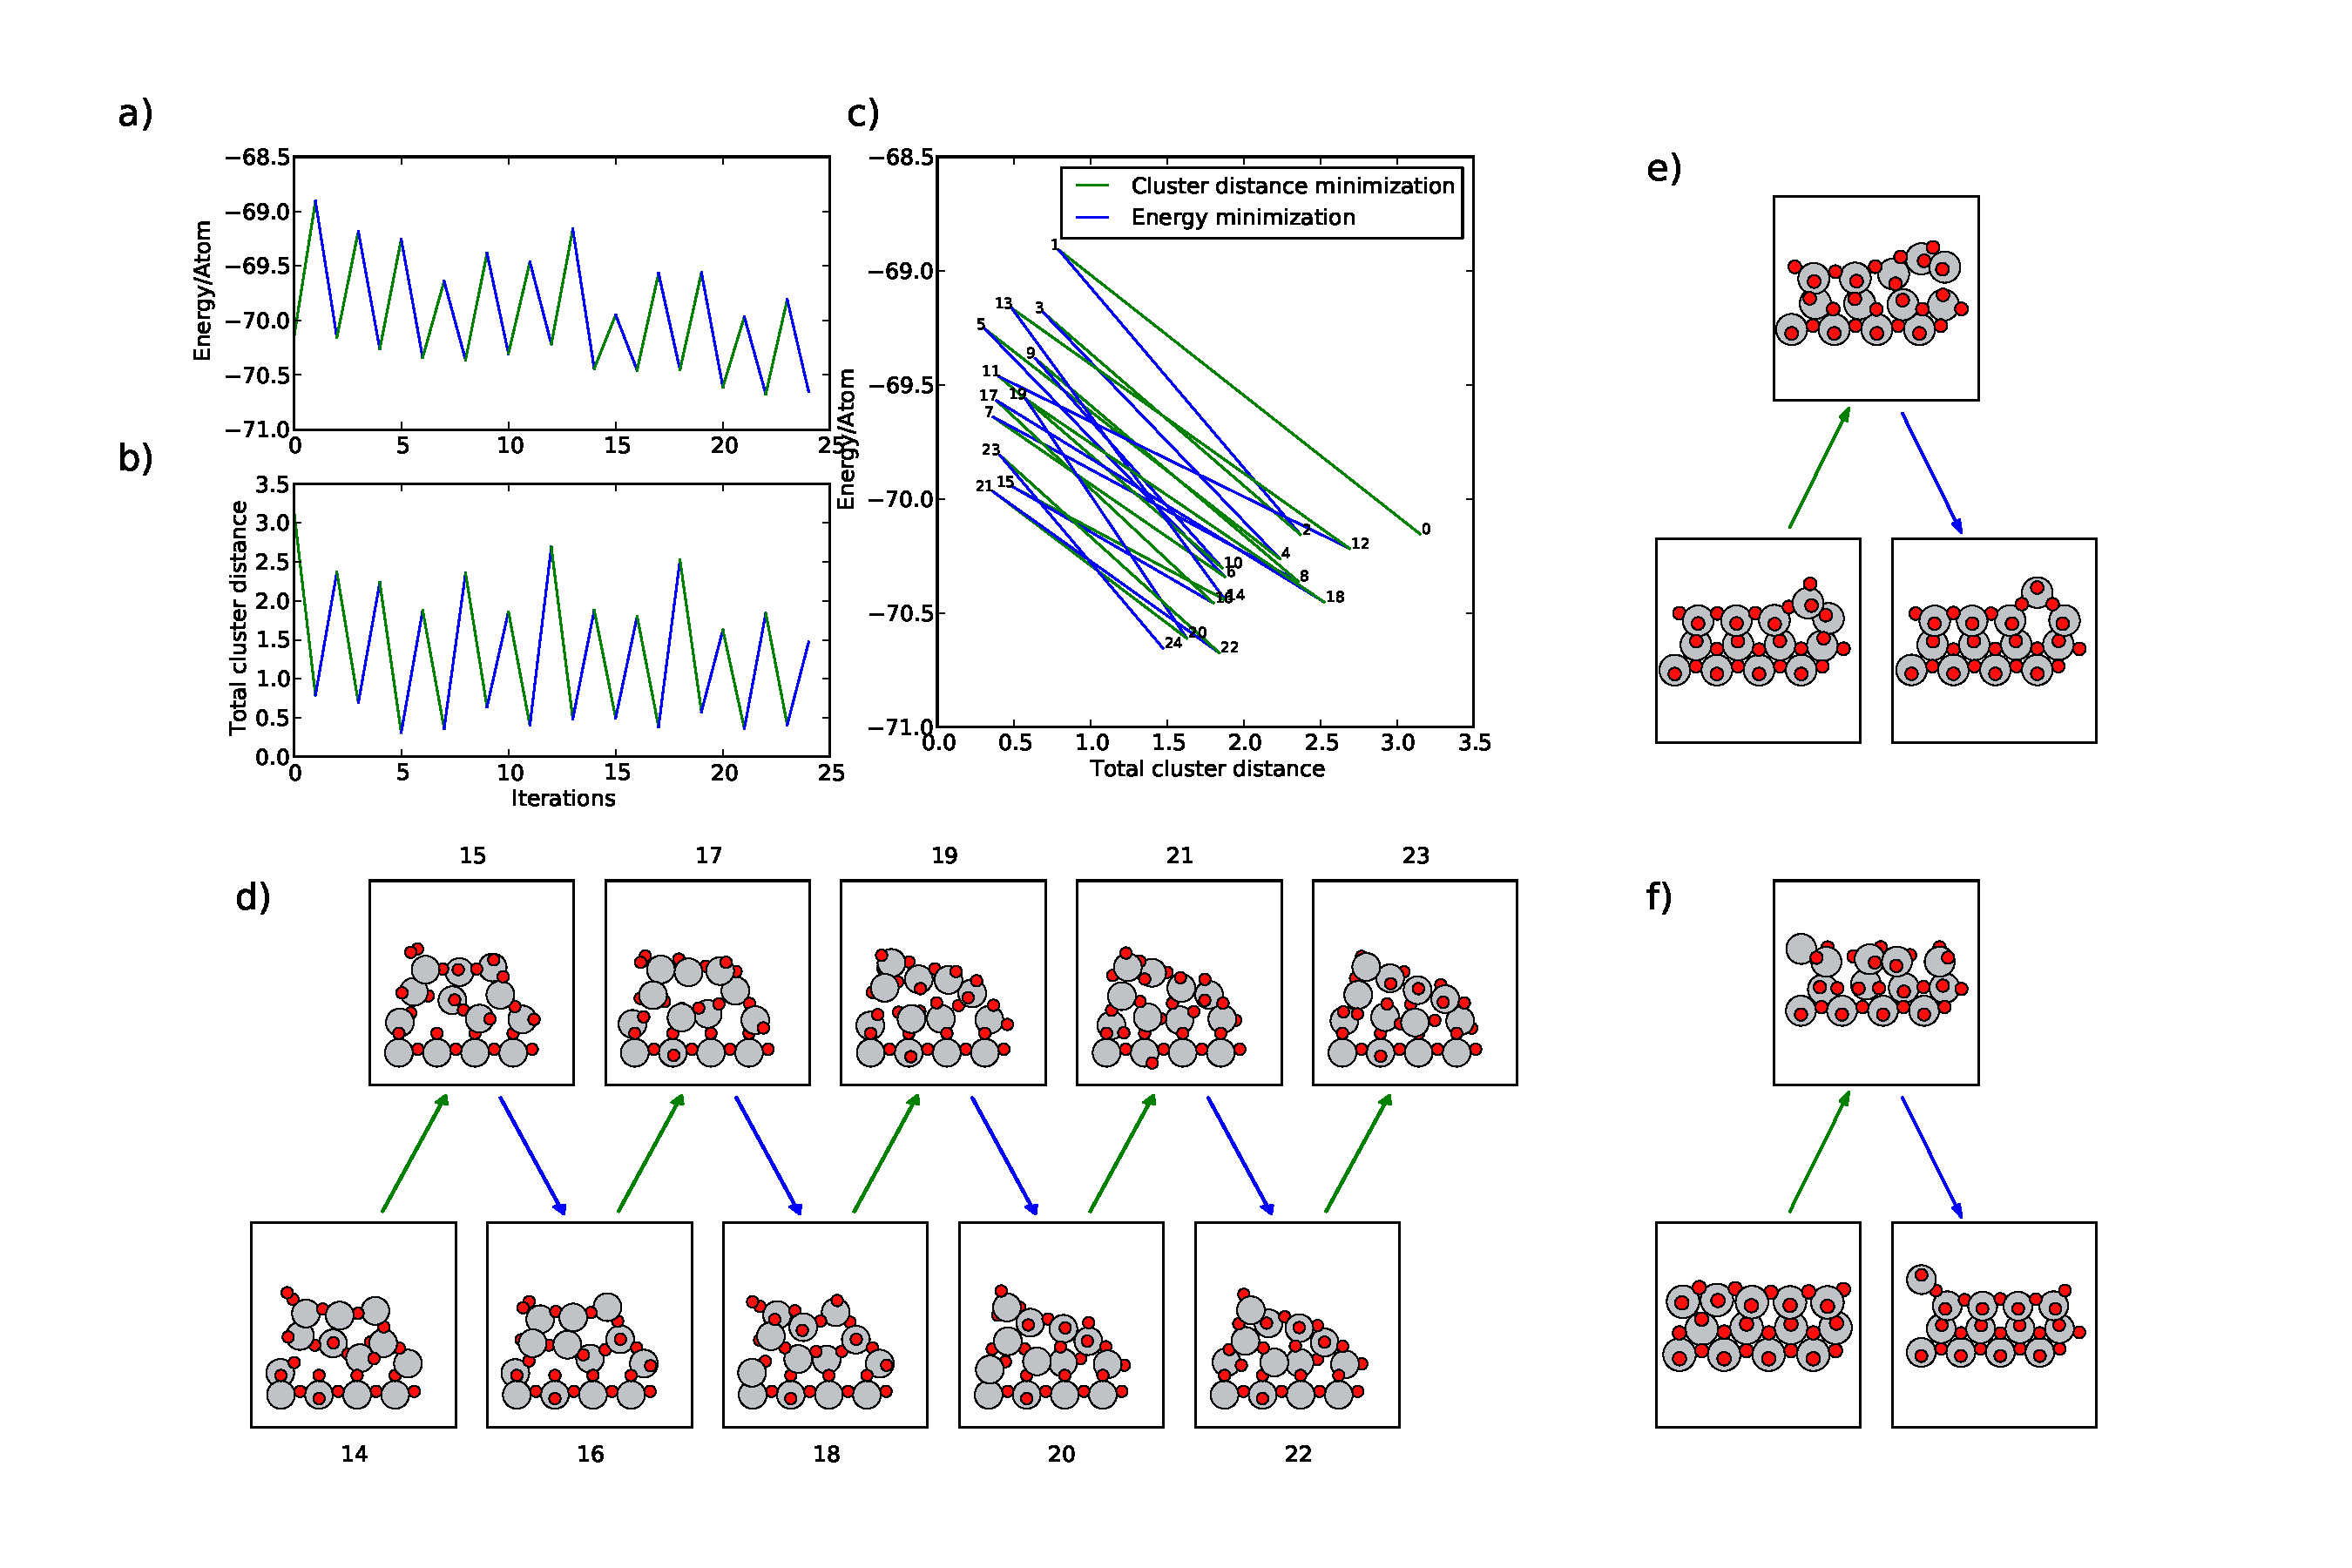
\includegraphics[width=2.0\columnwidth]{fig5-minimize.pdf}
    \caption{Green lines and arrows indicate cluster distance (cd) minimization steps, and blue lines indicate DFTB+ relaxations. Here the first (bottom) layer is the template. While it is hard to see progress in individual minimization steps there are small details to notice in the plot. In the cd step from 16 to 17 the vacancy in the second layer is filled and in the cd step from 18 to 19 the two oxygen atoms in the top left corner are split up.}
    \label{fig_min}
\end{figure*}

\subsubsection{Perturbation step in BH}
Figure \ref{fig_min} illustrates the outcome of the simplest
conceivable way of using the cluster regularization, namely as the
perturbing step in a basin hopping setup. In such a setup, the cluster
centers entering eq \ref{eq4} are obtained by clustering the
atomic features present in the latest structure of the search. Figures
\ref{fig_min}a-c illustrate how alternating cluster regularization
steps (green color) and local relaxation, i.e.\ energy minimization,
steps (blue color) lead to progressively more favorable
structures. Figures \ref{fig_min}a and b show the evolution of the
energy and the cluster distance, respectively, during the updates. The
starting point is a fully relaxed random structure which through the
cluster regularization perturbations is taken out of many different
local energy minima, thereby gaining about 0.5 eV/atom over the course of
25 updates. Figure \ref{fig_min}c combines the two measures, cluster
distance and energy, giving an overview of how the structure
develops. We observe (not shown) that many BH runs end up in the dynamic
equilibrium illustrated in Figure \ref{fig_schem}b. However, occasionally, the BH runs succeed in
identifying the global energy minimum structure, as illustrated with
the penultimate and ultimate optimization steps of such BH runs in
Figures \ref{fig_min}e-f.

\subsubsection{Mutation in EA}
The cluster regularization method lends itself particularly well for
use as a mutation in connection with an evolutionary algorithm (EA). It can
serve in a manner similar to that in a basin hopping setup, but owing
to the stochastic elements in the EA, the risk of being trapped in a
dynamic equilibrium is practically eliminated.

We introduced the cluster regularization as an EA mutation in the following way:
\begin{enumerate}
\item Draw randomly $N_\mathrm{par}$ parents from the population.
\item Calculate atomic features for all parents.
\item Cluster them and find cluster centers.
\item Minimize the cluster distance of the lowest energy parent
\item Return the resulting structure (the child)
\end{enumerate}
When the mutation returns the child, the EA will make an energy
relaxation and we have a cycle similar to that of the BH setup
illustrated in Figure \ref{fig_min}. However, for the EA cycle, the
random drawing of parents will ensure a more stochastic nature of the
search.

The optimum values of the free parameters in the new mutation were
determined with Bayesian hyper-parameter optimization (BHO) test runs on the three-layer system. We found $N_c=5$ clusters, $N_\mathrm{par}=3$
parents, and a cut-off radius of $r_c=11.9$ {\AA} as the optimum
values. Next, a separate BHO search was done to identify the optimum
frequency by which the mutation should be used. The search gave an
optimum ratio of 70\% cluster regularization, 28\% cut-and-splice, and 2\%
rattle mutation when cluster regularization was included, which
compares to a BHO result of 59\% cut-and-splice and
41\% rattle mutation in the absence of the cluster regularization. The
latter parameters were used for benchmark runs. In order to gauge the efficiency of
the cluster regularization method on its own we further did EA runs
using that method exclusively (i.e.\ having 100\% cluster
regularization and 0\% cut-and-splice and 0\% rattle mutation).

\begin{figure}[!hb]
    \centering
    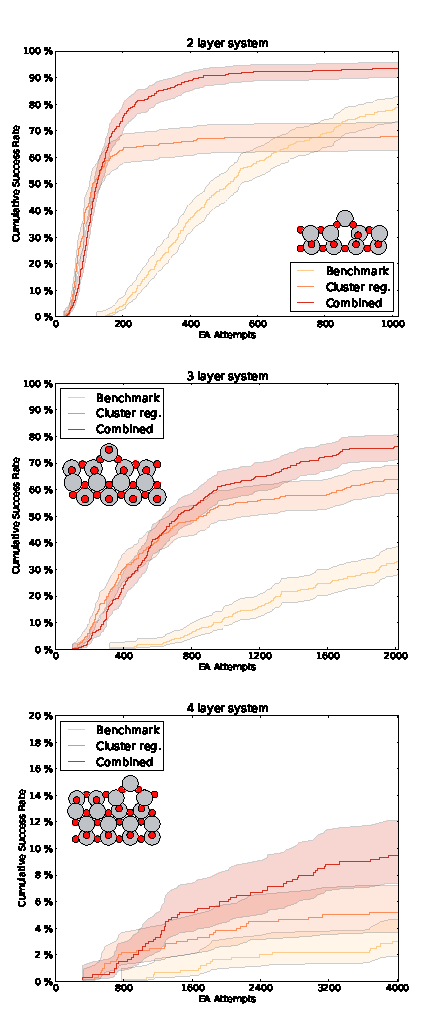
\includegraphics[width=1.0\columnwidth]{fig6-success.pdf}
    \caption{Cumulative success for 2,3 and 4 layer systems}
    \label{fig_success}
\end{figure}

\section{Global structure search results}


The three EA settings -- benchmark, all-cluster regularization, and
combined -- were tested for two-, three-, and four-layer TiO$_2$
systems. The results are presented in Figure \ref{fig_success} which
plot the accumulated success rates of XX restarts of the EA. Note that
the number of required attempts (measured on the $x$-axis) changes as
the system size increases.

For all system sizes, it is seen that the all-cluster regularization
method (orange curve) starts finding the global minimum energy
structure much sooner than the benchmark method (yellow curve). For the two-layer system,
the all-cluster regularization method levels off (i.e.\ stagnates) at around 60-70\%
success rate, which is smaller than what is obtained in the benchmark
runs. The larger systems were not run long enough to see if a similar
effect would occur for these systems. We speculate that the observed
stagnation of the all-cluster regularization can be explained as a set
of dynamic equilibria having been reached, now involving a large
number of structures (essentially most of the population members).

By resorting to the combined method, where the cluster regularization
method is used with its optimum 70\% likelihood, the overall best
performance is reached for all three systems (red curves). The
combined method still exhibits a much sooner onset of finding the global energy
minimum structure than the benchmark runs, and no signs of stagnation are seen.


\section{Summary}
In this work, we have used machine learning techniques to characterize
local atomic environments in structures found during structural
optimization of the anatase TiO$_2$(001) surface in search for the
global minimum energy structure, the (1$\times$4) ridge
reconstruction. Upon clustering according to feature vectors
describing the local atom environments, we find a correlation between
the sum of distances of the feature vectors to their respective
cluster centers for individual structures to the density functional
tight binding energies for these structures. The correlation enables
the formulation of a mutation operation for a basin hopping or
evolutionary algorithm that has a bias toward taking structures
into lower energy basins. The mutation minimizes the sum of the
distances to the cluster center by gradient based minimization
techniques. The usefulness of the mutation method is demonstrated in
evolutionary searches for the anatase TiO$_2$(001) (1$\times$4) ridge
reconstruction for three different system sizes.



\section{Acknowledgements}

We acknowledge support from the Danish Council for Independent Research | Natural Science (grant no. 0602-02566B) and from VILLUM FONDEN (Investigator grant, project no. 16562).

\begin{thebibliography}{12}  
\bibitem{Starke1998} U. Starke \textit{et al}., Phys. Rev. Lett. \textbf{80}, 758 (1998).    
\bibitem{Gilbert2006} K. M. Gilbert and C. A. Venanzi, {Hierarchical Clustering Analysis of Flexible GBR 12909 Dialkyl Piperazine and Piperidine Analogs} J. Comput. Aided Mol. Des. \textbf{20}, 209-225 (2006).  
\bibitem{Duan2010} L. L. Duan, Y. Mei, D. Zhang, Q. G. Zhang, and J. Z. H. Zhang, {Folding of a Helix at Room Temperature is Critically Aided by Electrostatic Polarization of Intraprotein Hydrogen Bonds} J. Am. Chem. Soc. \textbf{132}, 11159-11164 (2010).
\bibitem{Chema2003} D. Chema and A. Goldblum, {The "Nearest Single Neighbor" Method -- Finding Families of Conformations within a Sample} J. Chem. Inf. Comput. Sci. \textbf{43}, 208-217 (2003). 
\bibitem{Jorgensen2017} M. S. J{\o}rgensen, M. N. Groves, B. Hammer, {Combining Evolutionary Algorithms with Clustering toward Rational Global Structure Optimization at the Atomic Scale} J. Chem. Theory Comput. \textbf{13}, 1486-1493 (2017). 
\bibitem{Malay2009} {A Modified k-means Algorithm to Avoid Empty Clusters} Malay K. Pakhira, International Journal of Recent Trends in Engineering, Vol 1, No 1, May 2009
\bibitem{Pikard2011}  {Ab initio random structure searching} Chris J. Pickard and R. J. Needs. J. Phys.: Condens. Matter \textbf{23} (2011) 053201 (23pp) DOI:10.1088/0953-8984/23/5/053201
\bibitem{Botu2015} {Adaptive Machine Learning Framework to Accelerate Ab Initio Molecular Dynamics.} V. Botu and R. Ramprasad, Int. J. Quantum Chem. 2015, 115 ,1075-18083. DOI:10.1002/qua.24836    
\bibitem{Chen2017} {Understanding atomic chemistry with machine learning.} Chen, X., J�rgensen, M. S., Hammer, B., \& Li, J. (2017) Unpublished
\bibitem{Vilhelmsen2012}L. B. Vilhelmsen and B. Hammer, Phys. Rev. Lett. \textbf{108}, 126101 (2012).
\bibitem{Vilhelmsen2014}L. B.\ Vilhelmsen and B.\ Hammer, J. Chem. Phys. \textbf{141}, 044711 (2014).
\bibitem{ase2}A.\ H.\ Larsen \textit{et al.}, J. Phys. Condens. Matter 2017, 29, 273002.
\end{thebibliography}


\end{document}


